\subsection{Совместная работа против Германии и Турции}
В начале XX века Германия захотела связать прямым железнодорожным сообщением Берлин и Ормузский пролив.

{\centering 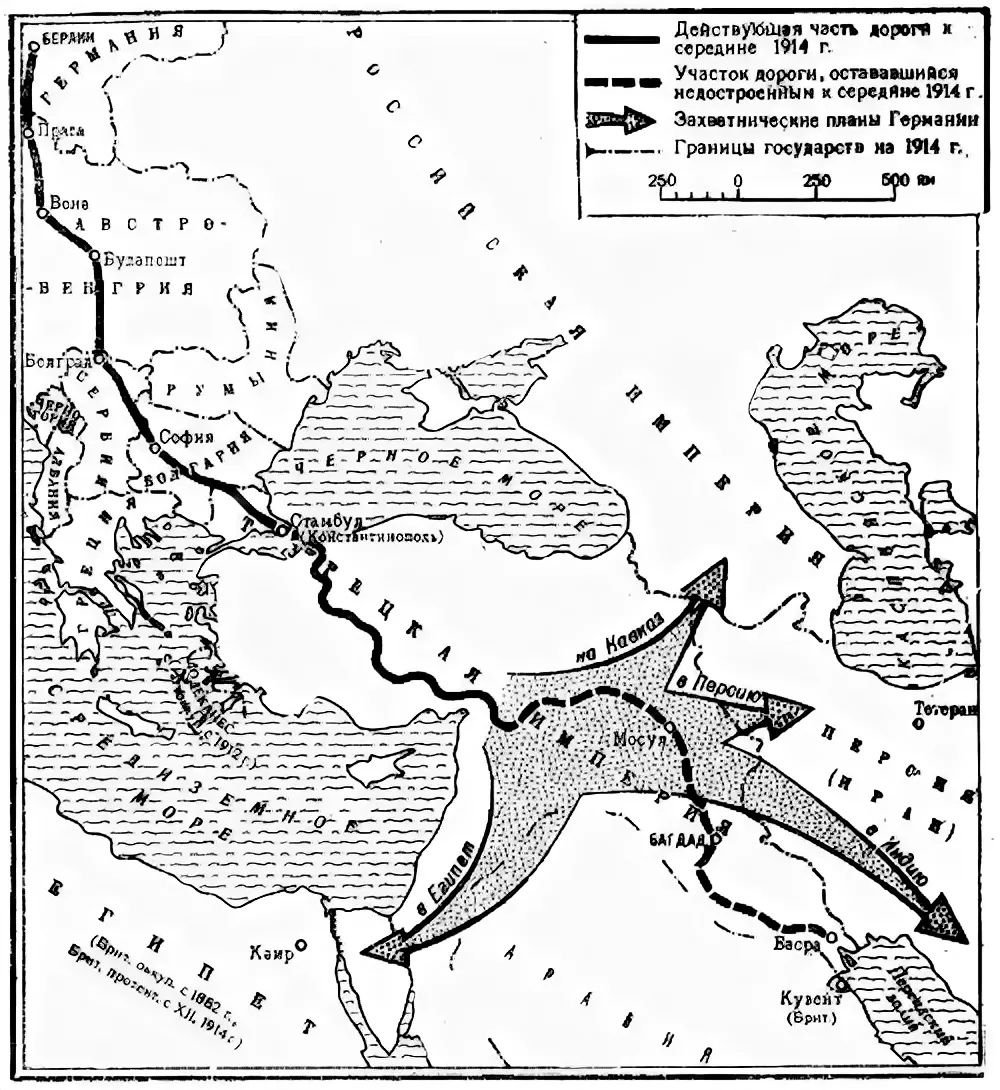
\includegraphics[width=\textwidth]{images/imgpreview.jpg}}

Это крайне не понравилось России и Великобритании, т.к. при завершении проекта Германия смогла бы получить выход в Индийский океан в обход Суэцкого канала и в обход Транс-сибирской магистрали, тем самым Российская и Английская теряла деньги, влияние на немецких промышленников, а следовательно и на Германию, помимо этого это означало бы распространение влияния на территории Ближнего Востока, который уже был поделен между Петроградом и Лондоном, поэтому страны всячески препятствовали данному проекту.